\subsection{Modelos basados en redes neuronales}

A partir de 1986\cite{Rumelhart_1987}, los modelos conexionistas o redes neuronales han sido utilizados como herramientas de predicción y clasificación. Un modelo basado en redes neuronales es un sistema informático que mediante el uso de pesado auto-modificable.

\paragraph{Perceptrón}

El perceptrón fue propuesto por Frank Rosenblatt\cite{Rosenblatt_1958}. El modelo más básico de una neurona es un perceptrón. El perceptrón usa una matriz para representar las redes neuronales, esta matriz es llamada matriz de pesos o solamente pesos. Las componentes de un modelo perceptrón son la capa de entrada, la capa oculta, una función de activación y la salida. En la capa oculta es donde se calcula la mutiplicación con la matriz de pesos. En la tabla \ref{table:activation_functions} se encuentran las funciones más usadas como funciones de activación.

\begin{table}[H]
	\centering
	\begin{tabular}{ll} \hline
		\textbf{Función} & \textbf{Definición}         \\ \hline
		Lineal           & $f(x)=x$                    \\[0.1cm]
		Sigmoide         & $f(x)=\frac{1}{1+e^{-x}}$   \\[0.1cm]
		ReLU             & $f(x)=\begin{cases}
				                         0 & \text{si x}<0     \\
				                         x & \text{si x}\leq 0 \\
			                         \end{cases}$ \\ [0.1cm]
		Tanh             & $f(x)=tanh(x)$              \\ [0.1cm] \hline
	\end{tabular}
	\caption{Funciones de activación comúnmente usadas.}
	\label{table:activation_functions}
\end{table}

El perceptrón multicapa tiene una estructura similar a la de un modelo perceptrón. En este caso se incluyen capas ocultas donde todas se encuentran conectadas, a esto se le denomina como una capa densa. En cada iteración existe una actualización con propagación hacia atras en las capas densas para entrenar el modelo. En nuestro caso se implemento un perceptrón multicapa con tres capas de 256, 128 y 3 capas densas con la función de activación sigmoide. En la figura \ref{fig:perceptron} se representa de manera visual el modelo perceptrón.
\begin{figure}[H]
	\centering
	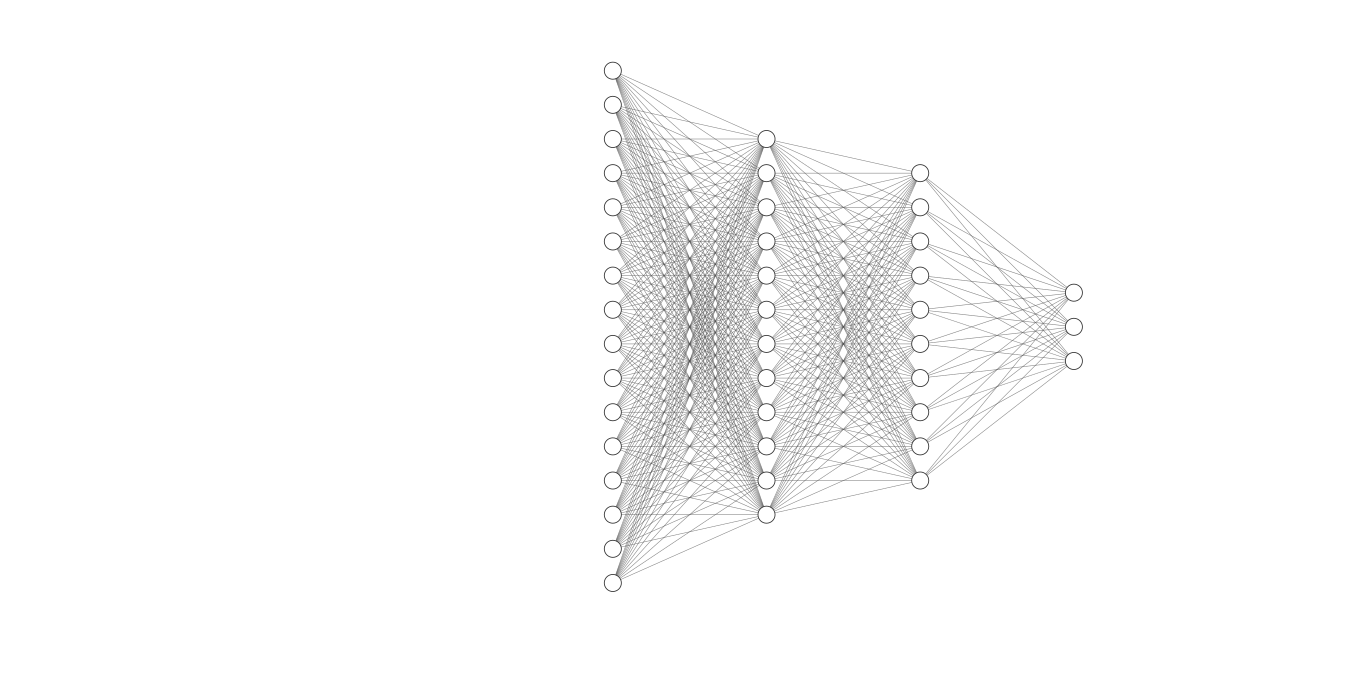
\includegraphics[width=8cm]{Graphics/perceptron.png}
	\caption{Representación del modelo perceptrón multicapa\cite{dotnet}.}
	\label{fig:perceptron}
\end{figure}
En la tabla \ref{table:perceptron} se muestra el número de parámetros y la salida y entrada de cada capa en el modelo creado.
\begin{table}[H]
	\centering
	\begin{tabular}{llr} \hline
		\textbf{Capa} & \textbf{Salida} & \begin{tabular}{c} \textbf{Número} \\ \textbf{de parámetros} \end{tabular} \\ \hline
		Flatten       & 24              & 0                                                                          \\
		Densa 1       & 256             & 6400                                                                       \\
		Densa 2       & 128             & 32896                                                                      \\
		Densa 3       & 3               & 387                                                                        \\ \hline
	\end{tabular}
	\caption{Estructura del modelo perceptrón implementado.}
	\label{table:perceptron}
\end{table}
\paragraph{Red Recurrente}
Las redes neuronales recurrentes (RNN) son una clase de redes neuronales que permiten conocer la salida anterior y utilizarla conociendo sus pesos. Para cada tiempo t, la función de activación ($a_t$) y la salida ($y_t$) pueden ser calculadas con las ecuaciones \ref{eq:rnn_a} y \ref{eq:rnn_y}.

\begin{minipage}{0.47\linewidth}

	\begin{equation}
		a_t = g_1(W_{aa}a_{t-1}+W_{ax}x_t+b_a)
		\label{eq:rnn_a}
	\end{equation}

\end{minipage}
\hspace{0.1cm}
\begin{minipage}{0.47\linewidth}

	\begin{equation}
		y_t = g_2(W_{ya}a_t+b_y)
		\label{eq:rnn_y}
	\end{equation}

\end{minipage}

En la figura \ref{fig:rnn} se visualiza a arquitectura de una RNN.

\begin{figure}[H]
	\centering
	\hspace*{2cm}
	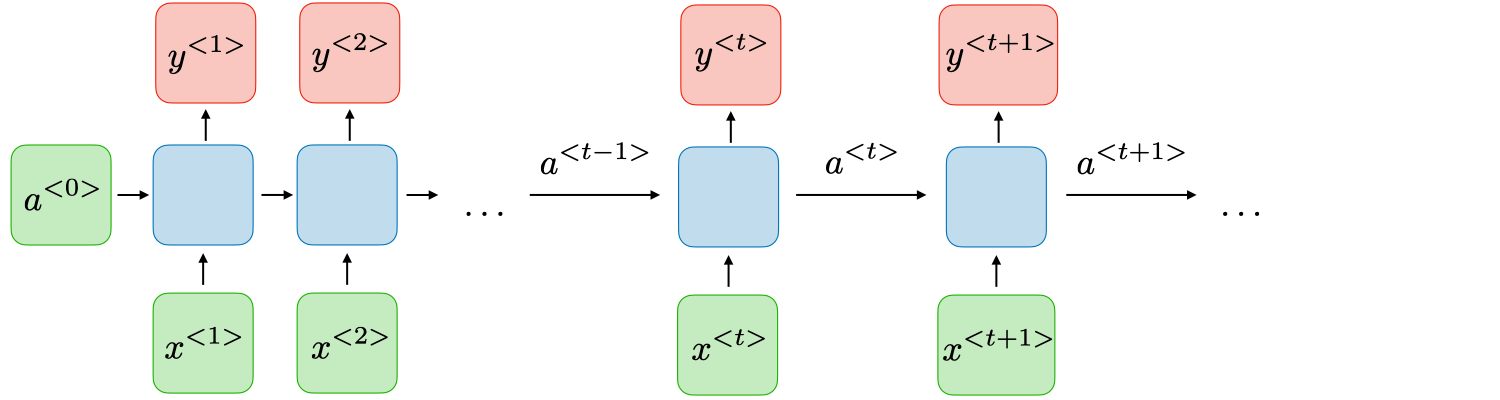
\includegraphics[width=15cm]{Graphics/rnn.png}
	\caption{Ilustración de una red neuronal recurrente\cite{rnn_image}.}
	\label{fig:rnn}
\end{figure}

En la tabla \ref{table:rnn} se muestra la estructura de la RNN creada para este proyecto. La capa RNN tiene como función de activación a la función ReLU y la capa densa una función sigmoide.

\begin{table}[H]
	\centering
	\begin{tabular}{llr} \hline
		\textbf{Capa} & \textbf{Salida} & \begin{tabular}{c} \textbf{Número} \\ \textbf{de parámetros} \end{tabular} \\ \hline
		RNN           & 64              & 4224                                                                       \\
		Densa         & 3               & 195                                                                        \\ \hline
	\end{tabular}
	\caption{Estructura del modelo RNN implementado.}
	\label{table:rnn}
\end{table}

\paragraph{Red Convolucional}

A diferencia de un modelo perceptrón, los modelos de redes neuronales convolucionales (CNN) consta de dos partes, una que se encarga del proceso de la convolución y otra del proceso de la predicción o la clasificación. En el proceso de convolución el objetivo es extraer la información mas relevante para la tarea. La operación convolución es comunmente usada para realizar transformaciones y obtener información de ella\cite{Unser_1995,Boellaard_1997,Hang_Gao_2009}. En nuestro caso, estamos tratandocon un vector, por ende la convolución que se aplica sera una restringuida en una dimensión. Después del proceso de las capas de convolución se obtienen una serie de vectores de una mayor dimensión, para reducir las mismas pasan por una capa llamada fully connected. La capa más común para realizar este proceso es llamada Max-polling, la cual dentro de una ventana en la serie de vectores obtiene unicamente el máximo. En la figura se muestra un ejemplo de esta capa en una matriz de 4x4.

\begin{figure}[H]
	\centering
	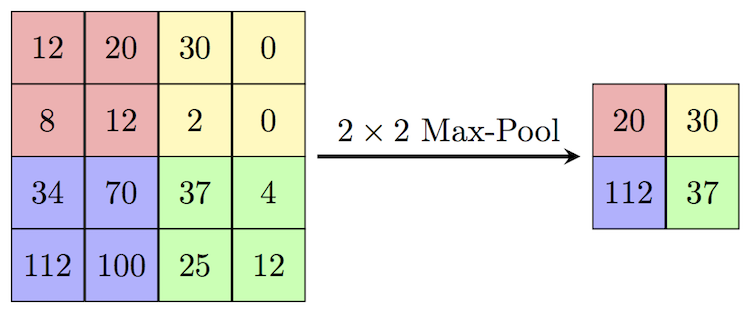
\includegraphics[width=7cm]{Graphics/maxpolling.png}
	\caption{Ejemplo de la capa Max-polling sobre una matriz de 4x4\cite{max_polling_image}.}
	\label{fig:maxpolling}
\end{figure}

En nuestro caso, en vez de usar una capa de Max-polling se implemento un capa de Global-Average-Polling\cite{min_2013}, la cual realiza un promedio de los vectores obtenidos a partir de todas las convoluciones obtenidas. En la figura \ref{fig:cnn} se muestra un ejemplo de una arquitectura de una CNN.

\begin{figure}[H]
	\centering
	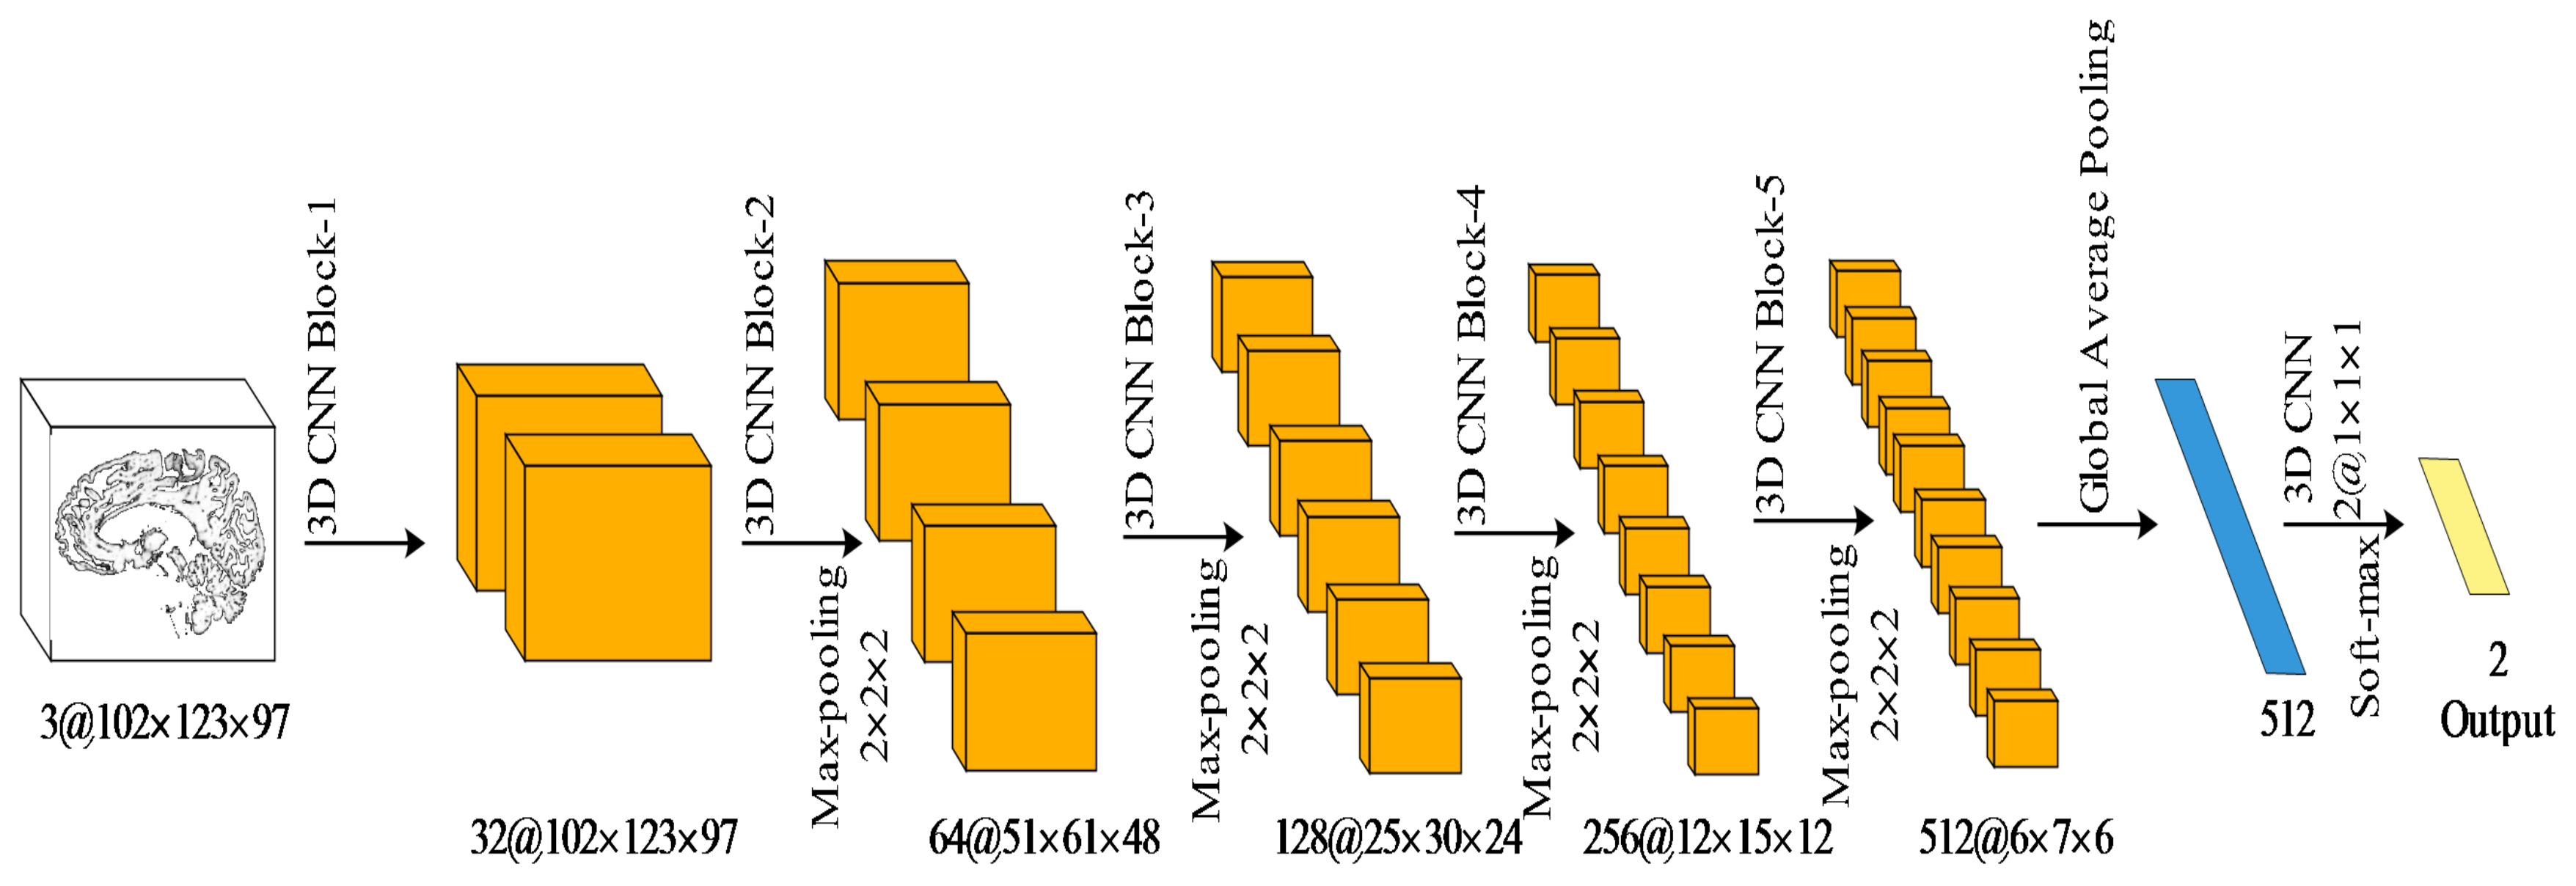
\includegraphics[width=14cm]{Graphics/cnn.png}
	\caption{Arquitectura de una CNN\cite{Qu_2020}.}
	\label{fig:cnn}
\end{figure}

En la tabla \ref{table:cnn} se muestra la estructura del modelo CNN implementado. Las capas convoluciones tienen como función de activación a la función ReLU y la capa densa la función sigmoide.

\begin{table}[H]
	\centering
	\begin{tabular}{llr} \hline
		\textbf{Capa}  & \textbf{Salida} & \begin{tabular}{c} \textbf{Número} \\ \textbf{de parámetros} \end{tabular} \\ \hline
		Conv1D 1       & 22,100          & 400                                                                        \\
		Conv1D 2       & 20,200          & 60200                                                                      \\
		Conv1D 3       & 18,200          & 120200                                                                     \\
		Global Average & 200             & 0                                                                          \\
		Densa          & 3               & 603                                                                        \\ \hline
	\end{tabular}
	\caption{Estructura del modelo CNN implementado.}
	\label{table:cnn}
\end{table}


\paragraph{Long short-term memory}

El modelo long short-term memory (LSTM) es una red neuronal la cual contiene propagación hacia atras semejante a las RNN. La red LSTM es creaada para modificar una característica de la red RNN. La característica que se modificada es que en el momento t, el estado oculto de los tiempos anteriores tienen una atribución menor conforme avanza el tiempo. Una red LSTM preserva la contribución de datos importantes independientemente de cuando aparezca. Por lo tanto, puede tener una memoria de corto y largo plazo. En la figura se muestra una celda de la red LSTM. A diferencia de una celda de una red RNN, la LSTM contiene un elemento adicional llamado celda de estado ($c_t$) . La celda de estado es la encargada de preservar la información relevante en cualquier tiempo.

\begin{figure}[H]
	\centering
	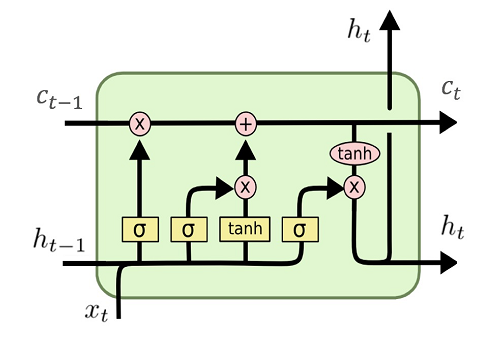
\includegraphics[width=8cm]{Graphics/lstm.png}
	\caption{Celda de la red LSTM con sus elementos\cite{lstm_image}.}
	\label{fig:lstm}
\end{figure}

En la tabla \ref{table:lstm} se encuentra la estructura de la red LSTM implementada. La capa densa tiene como función de ativación la función sigmoide.

\begin{table}[H]
	\centering
	\begin{tabular}{llr} \hline
		\textbf{Capa} & \textbf{Salida} & \begin{tabular}{c} \textbf{Número} \\ \textbf{de parámetros} \end{tabular} \\ \hline
		LSTM 1        & 24,256          & 264192                                                                     \\
		LSTM 2        & 256             & 525312                                                                     \\
		Densa         & 3               & 771                                                                        \\ \hline
	\end{tabular}
	\caption{Estructura del modelo LSTM implementado.}
	\label{table:lstm}
\end{table}

\paragraph{Bidireccional Long-short-term memory}

El modelo Bidireccional Long short-term memory (Bi-LSTM) añade la característica de analizar los datos de entrada hacia delante y hacia atras. En la figura \ref{fig:bi_lstm} se muestra la estructura interna de una red Bi-LSTM.

\begin{figure}[H]
	\centering
	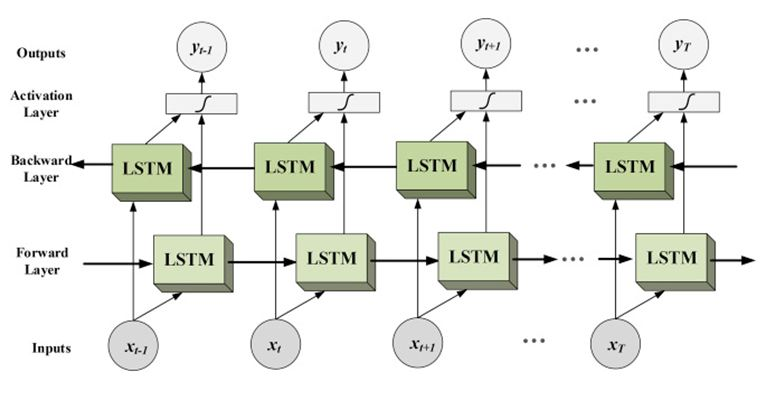
\includegraphics[width=10cm]{Graphics/bi_lstm.jpg}
	\caption{Estructura interna de la red Bi-LSTM\cite{bilstm_image}.}
	\label{fig:bi_lstm}
\end{figure}

En la tabla \ref{table:bi_lstm} se muestra la estructura interna del modelo Bi-LSTM implementado.

\begin{table}[H]
	\centering
	\begin{tabular}{llr} \hline
		\textbf{Capa} & \textbf{Salida} & \begin{tabular}{c} \textbf{Número} \\ \textbf{de parámetros} \end{tabular} \\ \hline
		Bi-LSTM 1     & 24,512          & 528384                                                                     \\
		Bi-LSTM 2     & 512             & 1574912                                                                    \\
		Densa         & 3               & 1539                                                                       \\ \hline
	\end{tabular}
	\caption{Estructura del modelo Bi-LSTM implementado.}
	\label{table:bi_lstm}
\end{table}


\paragraph{Red convolucional con atención}

La atención es una técnica que toma la idea de la atención cognitiva de los humanos. La idea principal es que el modelo se enfoque en cierta parte de la entrada e ignore la otra, esto por medio de un sistema de pesado. El uso de multiples mecanismos de atención afronta la desventaja que tiene la convolución\cite{Yunpeng_2018,Yunpeng_2019}. Es por ello, que se implemento esta capa de atención en la estructura de la red CNN descrita en la tabla \ref{table:cnn}. En la tabla \ref{table:cnn_with_attention} se encuentra la estructura de la red CNN con atención implementada.

\begin{table}[H]
	\centering
	\begin{tabular}{llr} \hline
		\textbf{Capa}  & \textbf{Salida} & \begin{tabular}{c} \textbf{Número} \\ \textbf{de parámetros} \end{tabular} \\ \hline
		Conv1D 1       & 20,100          & 600                                                                        \\
		Conv1D 2       & 18,200          & 60200                                                                      \\
		Conv1D 3       & 16,200          & 120200                                                                     \\
		Global Average & 32              & 52800                                                                      \\
		Densa          & 3               & 99                                                                         \\ \hline
	\end{tabular}
	\caption{Estructura del modelo CNN con atención implementado.}
	\label{table:cnn_with_attention}
\end{table}

\paragraph{Esquema de votación}

En base a los modelos neuronales implementados, se desarrollo un esquema de votación en el cual se seleccionan a los tres mejores modelos en base a su precisión para cada estación y se realiza una media aritmética de su resultado final.
